% !TEX encoding = UTF-8 Unicode

\documentclass[a4paper]{article}

\usepackage{color}
\usepackage{url}
\usepackage[T2A]{fontenc} % enable Cyrillic fonts
\usepackage[utf8x]{inputenc} % make weird characters work
\usepackage{graphicx}
\usepackage{caption}
\usepackage{subcaption}
\usepackage{float}
\usepackage[section]{placeins}
\usepackage[english,serbian]{babel}
\usepackage{color}
%\usepackage[english,serbianc]{babel} %ukljuciti babel sa ovim opcijama, umesto gornjim, ukoliko se koristi cirilica

\usepackage[unicode]{hyperref}
\hypersetup{colorlinks,citecolor=green,filecolor=green,linkcolor=blue,urlcolor=blue}

%\newtheorem{primer}{Пример}[section] %ćirilični primer
\newtheorem{definicija}{Definicija}[section]

\begin{document}

\title{ATP 2000-2017\\ \small{Seminarski rad u okviru kursa\\Istraživanje podataka\\ Matematički fakultet}}

\author{Marija Mijailović\\ mi14199@alas.matf.bg.ac.rs\\Miroslav Mišljenović\\mr12260@alas.matf.bg.ac.rs}
\date{jun 2018.}
\maketitle

\abstract{
U ovom radu analizirali smo skup podataka ˝ATP - rezultati turnira od 2000-2017˝. Obradili smo pravila pridruživanja, klasterovanje, klasifikaciju i predstavili sve navedene metode odgovarajućom vizualizacijom. Skup podataka je preuzet sa \url{https://www.kaggle.com/gmadevs/atp-matches-dataset}.
}

\tableofcontents

%\newpage

\section{Uvod}
\label{sec:uvod}

Skup podataka ATP mečeva podeljen je u 17 zasebnih .csv fajlova i svaki od njih prikazuje individualne statistike za svaki turnir u toku te godine.

%Na Slici \ref{fig:picture1}(b) prikazana je jednostavna mrežna toppologija, sastavljena od 4 rutera označenih sa A, B, C i D. Ruteri B i C su povezani sa spoljašnjom mrežom Ext, a ruter D je povezan sa dve unutrašnje mreže N1 i N2. U nastavku, pojam klase saobraćaja se odnosi na skup paketa (npr. paketi namenjeni N1) koji se obrađuju prema zahtevima. 
%\begin{figure}[h!]
%	\begin{center}
%		\includegraphics[scale=0.50]{resources/picture1.png}
%	\end{center}
%	\caption{Sinteza konfiguracije na mreži. Ulaz je: (a) deklarativna mrežna specifikacija N u Datalogu (b) topologija mreže, i (c) uslovi za rutiranje $ \phi\_{R} $. Izlaz je: (d) Datalog ulaz I koji rezultira u sledeće stanju koje zadovoljava zahteve. Konfiguracije (e) su izvedene iz I.}
%	\label{fig:picture1}
%\end{figure}

\section{Analiza podataka}

U ovom poglavlju sledi kratak pregled najistaknutijih atributa ovog skupa podataka.
Svaki red u skupu, označava jedan meč i sve informacije o tom meču.

U tabeli \ref{table:turnir} prikazani su podaci o turniru.
\begin{table}
		\begin{tabular}{ | c | c | } 
			\hline
			Ime kolone & Objašnjenje \\ 
			\hline
			tourney\_id & id turnira \\
			tourney\_name & ime turnira \\
			surface & podloga(Grass, Clay, Hard) \\
			tourney\_level & nivo turnira(Grand Slam, Finals, Masters, Tour Series, Challenger) \\ 
			round & runda(Round of 16, Quarterfinal...) \\
			minutes & trajanje meča u minutima \\
			\hline
		\end{tabular}
	\caption{Podaci o turnirima}
	\label{table:turnir}
\end{table}

U tabeli \ref{table:pobednici} prikazani su podaci o pobedniku meča.
\begin{table}
		\begin{tabular}{ | c | c | } 
			\hline
			Ime kolone & Objašnjenje \\ 
			\hline
			winner\_seed & nosilac na turniru \\
			winner\_entry & ulaznica(WildCard, Qualified, LuckyLoser, ProtectedRanking) \\
			winner\_name & ime pobednika \\
			winner\_ht & visina pobednika \\
			winner\_ioc & zemlja porekla pobednika \\
			winner\_age & godine pobednika \\
			winner\_rank & ATP rang pobednika \\
			winner\_rank\_points & ATP poeni pobednika \\
			w\_ace & broj asova pobednika \\
			w\_df & broj duplih grešaka pobednika \\ 
			w\_svpt & broj poena dobijenih na servis pobednika \\
			w\_1stIn & broj ubačenih prvih servisa pobednika \\
			w\_1stWon & broj poena dobijenih nakon ubačenog prvog servisa pobednika \\
			w\_2ndWon & broj poena dobijenih nakon ubačenog drugog servisa pobednika \\
			w\_SvGms & broj gemova u kojima je servirao pobednik \\
			w\_bpSaved & broj spašenih brejk šansi pobednika \\
			w\_bpFaced & broj brejk šansi na servis pobednika \\ 
			\hline
		\end{tabular}
	\caption{Podaci o pobednicima}
	\label{table:pobednici}
\end{table}

U tabeli \ref{table:gubitnici} prikazani su podaci o gubitniku meča.
\begin{table}
		\begin{tabular}{ | c | c | } 
			\hline
			Ime kolone & Objašnjenje \\ 
			\hline
			loser\_seed & nosilac na turniru \\
			loser\_entry & ulaznica(WildCard, Qualified, LuckyLoser, ProtectedRanking) \\
			loser\_name & ime gubitnika \\
			loser\_ht & visina gubitnika \\
			loser\_ioc & zemlja porekla gubitnika \\
			loser\_age & godine gubitnika \\
			loser\_rank & ATP rang gubitnika \\
			loser\_rank\_points & ATP poeni gubitnika \\ 
			l\_ace & broj asova gubitnika \\
			l\_df & broj duplih grešaka gubitnika \\
			l\_svpt & broj poena dobijenih na servis gubitnika \\
			l\_1stIn & broj ubačenih prvih servisa gubitnika \\
			l\_1stWon & broj poena dobijenih nakon ubačenog prvog servisa gubitnika \\
			l\_2ndWon & broj poena dobijenih nakon ubačenog drugog servisa gubitnika \\
			l\_SvGms & broj gemova u kojima je servirao gubitnik \\
			l\_bpSaved & broj spašenih brejk šansi gubitnika \\
			l\_bpFaced & broj brejk šansi na servis gubitnika \\
			\hline
		\end{tabular}
	\caption{Podaci o gubitnicima}
	\label{table:gubitnici}
\end{table}

S obzirom na veliki broj raspoloživih godina, prvo smo se detaljno upoznali sa podacima, šta nam koja godina pruža i koji su najzanimljiviji atributi za svaku godinu. U zavisnosti od toga smo, po potrebama metoda, koristili različite godine, ali svuda smo se ograničili na četiri maksimalno.

\section{Pravila pridruživanja}

Pravila pridruživanja smo obradili u programskom alatu KNIME (slika \ref{fig:knime}).
Odlučili smo se za 2009. godinu, jer su rezultati reprezentativniji u odnosu na ostale godine.

\begin{figure}[h!]
	\begin{center}
		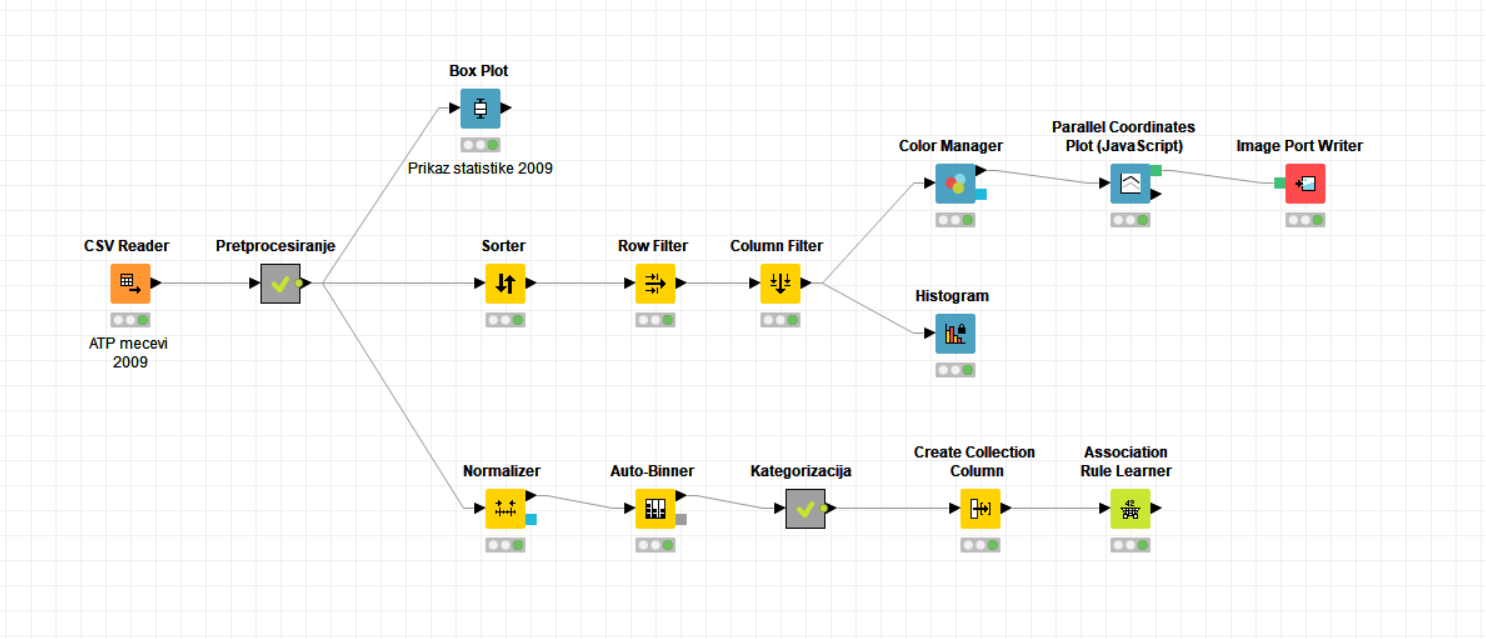
\includegraphics[scale=0.37]{KNIME_project/PravilaPridruzivanja/knime.png}
	\end{center}
	\caption{KNIME implementacija}
	\label{fig:knime}
\end{figure}

Na slikama \ref{fig:histogram} i \ref{fig:parallel} grafički su prikazani rezultati za sedam
tenisera koji su imali prosečno najviše asova po meču na kome su pobedili. Izabrali smo četiri parametra za svakog igrača:
broj asova pobednika, broj dobijenih poena na servis pobednika, broj ubačenih prvih servisa pobednika i
broj osvojenih poena nakon ubačenog prvog servisa pobednika. Na histogramu i grafiku paralelnih koordinata 
mogu se videti i uporediti rezultati.

\begin{figure}[H]
	\begin{center}
		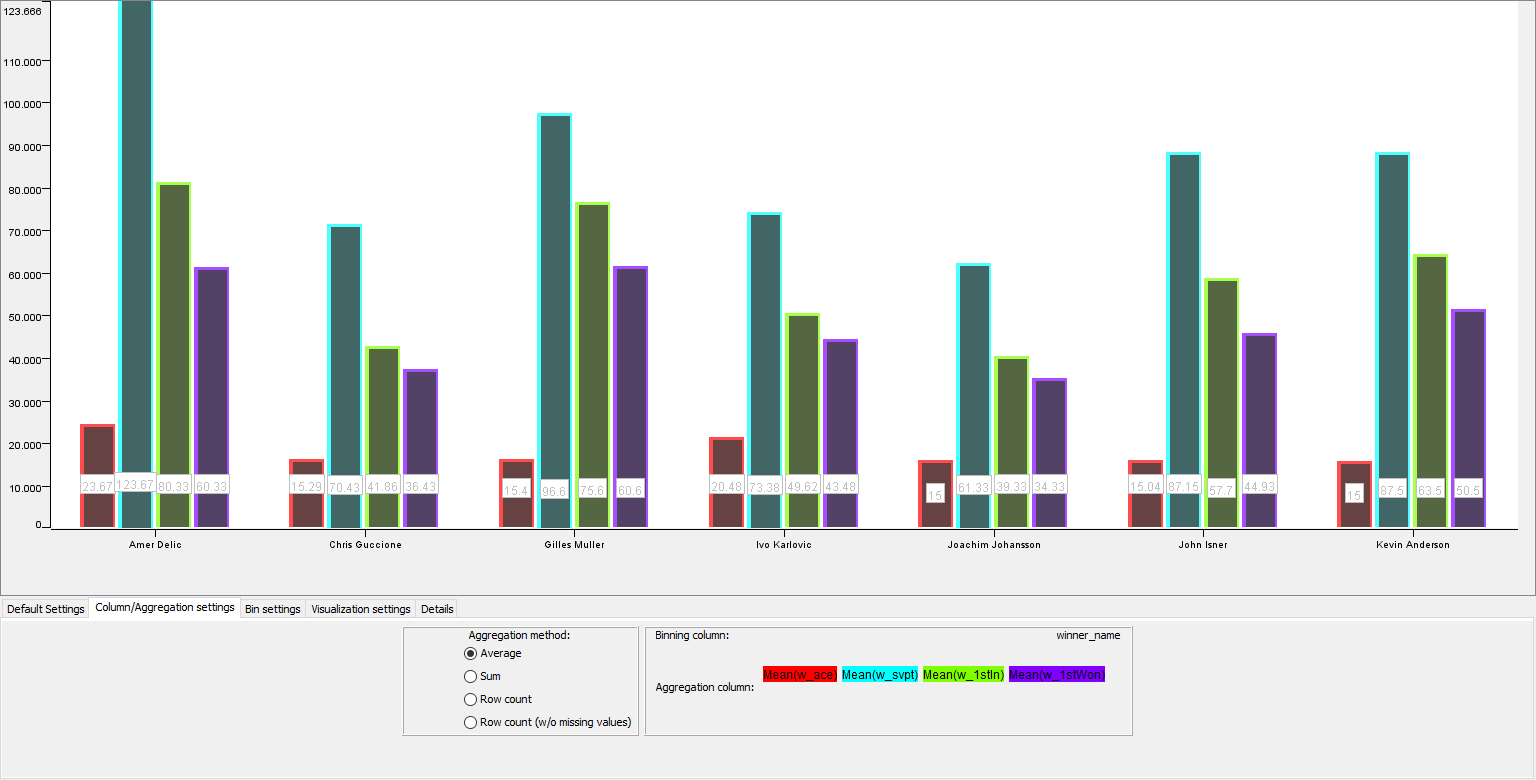
\includegraphics[scale=0.22]{KNIME_project/PravilaPridruzivanja/histogram2009}
	\end{center}
	\caption{Histogram}
	\label{fig:histogram}
\end{figure}

\begin{figure}[H]
	\begin{center}
		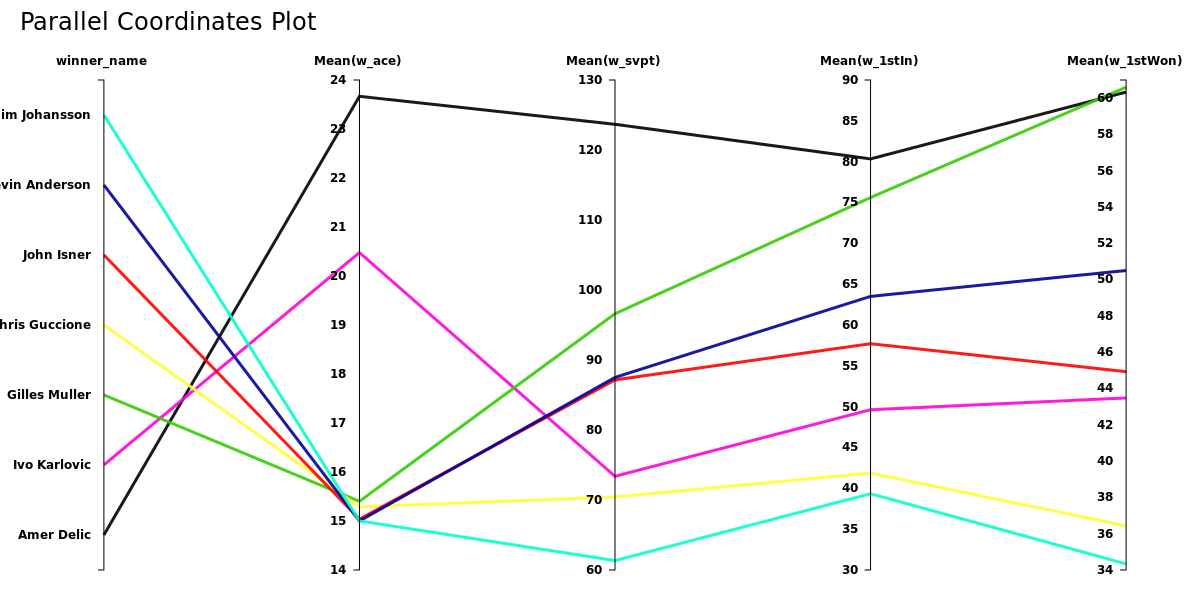
\includegraphics[scale=0.30]{KNIME_project/PravilaPridruzivanja/parallel2009}
	\end{center}
	\caption{Paralelne koordinate}
	\label{fig:parallel}
\end{figure}

Iznenađenje je pojavljivanje Amera Delića u prvih sedam, jer je to
autorima nepoznat igrač. Uvidom u podatke, utvrđeno je da je on te godine odigrao samo osam mečeva,
a pobedio je samo tri puta, u mečevima u kojima je imao mnogo asova (što je kriterijum po kome je birano najboljih sedam). \\

U tri kategorije smo podelili sledeća četiri atributa: broj asova pobednika, broj duplih servis grešaka pobednika,
broj osvojenih poena nakon ubačenog prvog servisa pobednika, broj spašenih brejk lopti pobednika.
Na slici \ref{fig:rule_learner} se mogu videti pravila pridruživanja dobijena na osnovu te kategorizacije,
sortirani po Lift meri. Za pouzdanost smo uzeli vrednost 0.4, a za minimalnu podršku vrednost 0.15.
Analizirali smo podatke za sve godine i rezultati su prilično uniformni. Za 2009. godinu je dobijena druga najveća
Lift mera (1.36) i odnosi se na pravilo [ACE 2, WON 2, DF 1] -> [BPS 1].
U 2004. godini smo dobili najveću vrednost Lift mere (1.441) za pravilo [BPS 1, ACE 1, DF 1] -> [WON 1].


\begin{figure}[h!]
	\begin{center}
		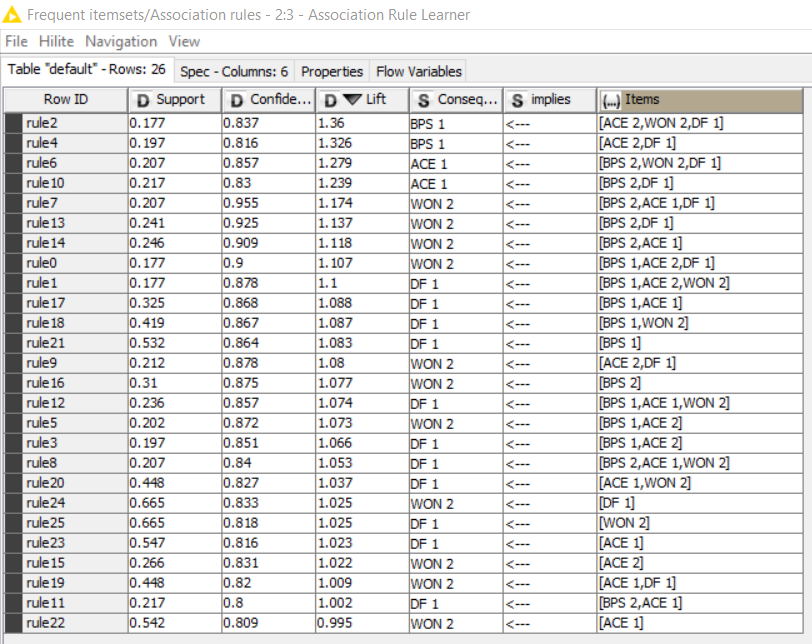
\includegraphics[scale=0.6]{KNIME_project/PravilaPridruzivanja/rule_learner_2009}
	\end{center}
	\caption{Pravila pridruživanja}
	\label{fig:rule_learner}
\end{figure}

\section{Klasterovanje}

Što se tiče klasterovanja, s obzirom da podaci po godinama dosta osciliraju, odlučili smo da klasterovanje izvršimo za više godina. Izabrali smo 2003., 2011. i 2017. godinu. Pre svega, zanimala nas je zavisnost broja godina pobednika i broj asova pobednika. Prvo smo obradili nedostajuće vrednosti. Klasterovanje smo obradili u alatima SPSS i KNIME (slike \ref{fig:SPSS_CvoroviKlasterovanje} i \ref{fig:KNIME_CvoroviKlasterovanje}). 

\subsection{SPSS}

\begin{figure}[H]
	\begin{center}
		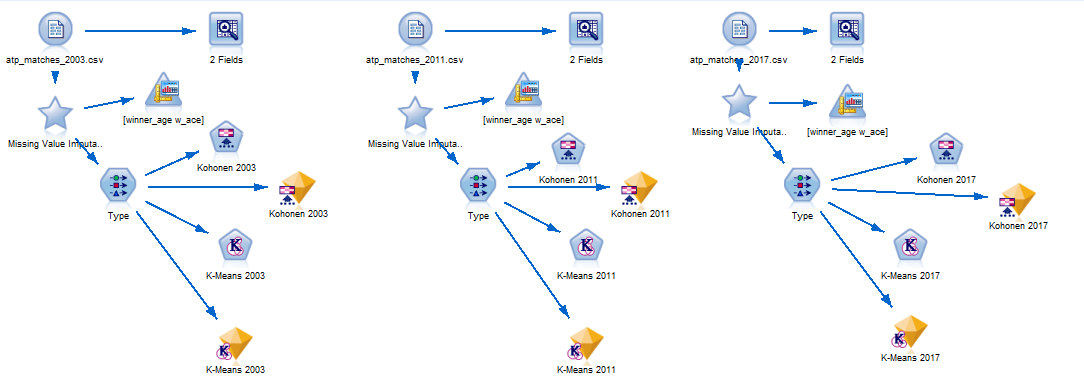
\includegraphics[scale=0.60]{Klasterovanje/SPSS_Cvorovi.png}
	\end{center}
	\caption{SPSS klasterovanje}
	\label{fig:SPSS_CvoroviKlasterovanje}
\end{figure}

U alatu SPSS smo pomoću siluete pratili kako nam se kvalitet klasterovanja razlikuje u zavisnosti od broja klastera. 
\textit{Kohonen} algoritam nam je za broj klastera između 3 i 5 davao ˝osrednji˝ kvalitet klasterovanja, pa ga nismo detaljno razmatrali. {\color{red} (Podseti me da probam sa nekim drugim ulaznim argumentima za Kohonena i da napisem ovde za koje smo probali.)} S druge strane, \textit{K-Means} algoritam nam je davao dosta raznolike ocene klastera po godinama. 2003. godina nam je za 4 i 5 klastera pokazala kvalitet klasterovanja  ˝dobar˝, uz važnost atributa \textit{w\_age = 1} i \textit{w\_ace = 1}. U 2011. godini nam je za 5 klastera silueta pokazivala kvalitet ˝osrednji˝, promenivši broj klastera na 4 silueta je prešla u ˝dobar˝. Takođe, i sa 4 klastera i sa 5 klastera važnost atributa \textit{w\_age = 1} i \textit{w\_ace = 1}. Rezultati za 2017. godinu za 4 klastera pokazuju kvalitet ˝osrednji˝; promenivši broj klastera na 5, silueta je na granici ˝osrednji˝-˝dobar˝, međutim, važnost atributa sa 4 klastera je \textit{w\_age = 1}, \textit{w\_ace = 0.77}, dok je sa 5 klastera \textit{w\_ace} opao na 0.46. Ipak smo odlučili da 2017. godinu odbradimo sa 5 klastera. Konačno, odlučili smo se za broj i kvalitet klastera koji su prikazani na slici \ref{Siluete}.

\begin{figure}[H]
	\begin{subfigure}[h]{\textwidth}
		\begin{center}
			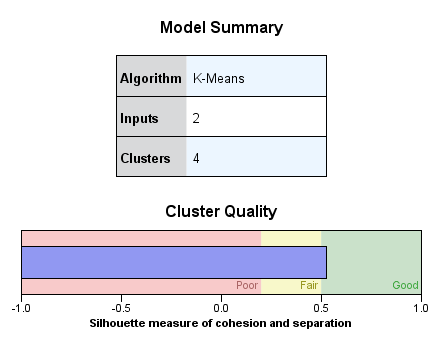
\includegraphics[scale=0.50]{Klasterovanje/Model_KMeans2003_Silhouette.png}
		\end{center}
		\caption{2003. godina}
		\label{fig:SPSS_Silueta2003}
	\end{subfigure}

	\vspace{0.5cm}
	\begin{subfigure}[h]{\textwidth}
		\begin{center}
			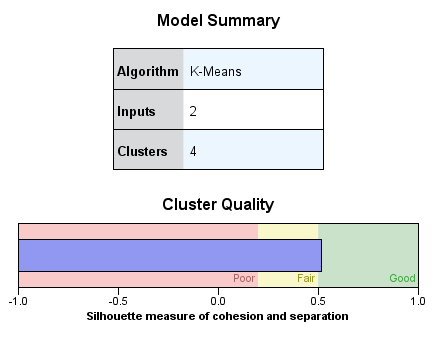
\includegraphics[scale=0.50]{Klasterovanje/Model_KMeans2011_Silhouette.png}
		\end{center}
		\caption{2011. godina}
		\label{fig:SPSS_Silueta2011}
	\end{subfigure}
	
	\vspace{0.5cm}
	\begin{subfigure}[h]{\textwidth}
		\begin{center}
			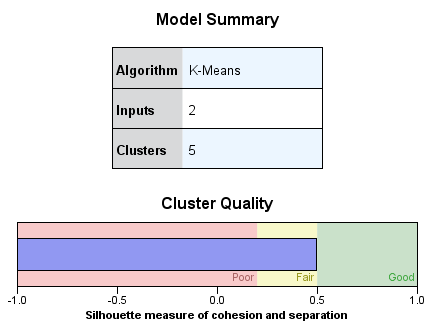
\includegraphics[scale=0.50]{Klasterovanje/Model_KMeans2017_Silhouette.png}
		\end{center}
		\caption{2017. godina}
		\label{fig:SPSS_Silueta2017}
	\end{subfigure}
	
	\caption{Kvalitet klasterovanja}
	\label{Siluete}
\end{figure}

Kao što se vidi na slici \ref{ModeliKlastera}, u sve tri godine su dobijeni interesantni podaci. Na primer, u 2003. godini najstariji igrači imaju slabiji prosek asova, dok u 2011. i 2017. godini imamo dva klastera sa prosekom godina oko 30; u jednom klasteru nam je broj asova mali, dok je u drugom najveći. Ovo nam je govorilo da možda imamo neki element van granica, koji je uticao na kreiranje dodatnog klastera. Odlučili smo da proverimo šta ćemo dobiti u KNIME-u.

\begin{figure}[H]
	\begin{subfigure}[h]{\textwidth}
		\begin{center}
			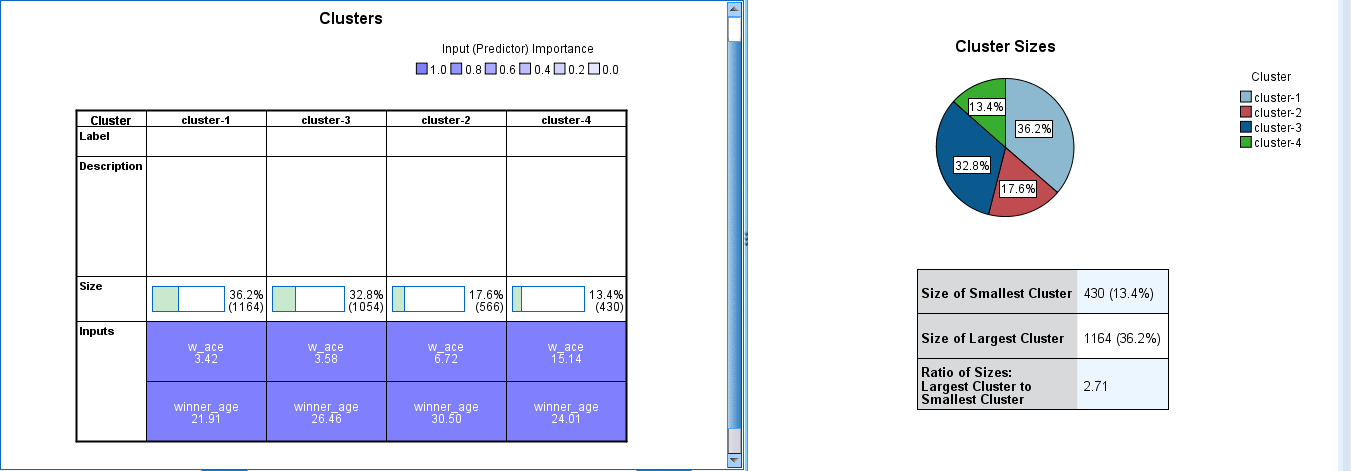
\includegraphics[scale=0.50]{Klasterovanje/Model_KMeans2003.png}
		\end{center}
		\caption{2003. godina}
		\label{fig:SPSS_Model2003}
	\end{subfigure}
	
	\vspace{0.5cm}
	\begin{subfigure}[h]{\textwidth}
		\begin{center}
			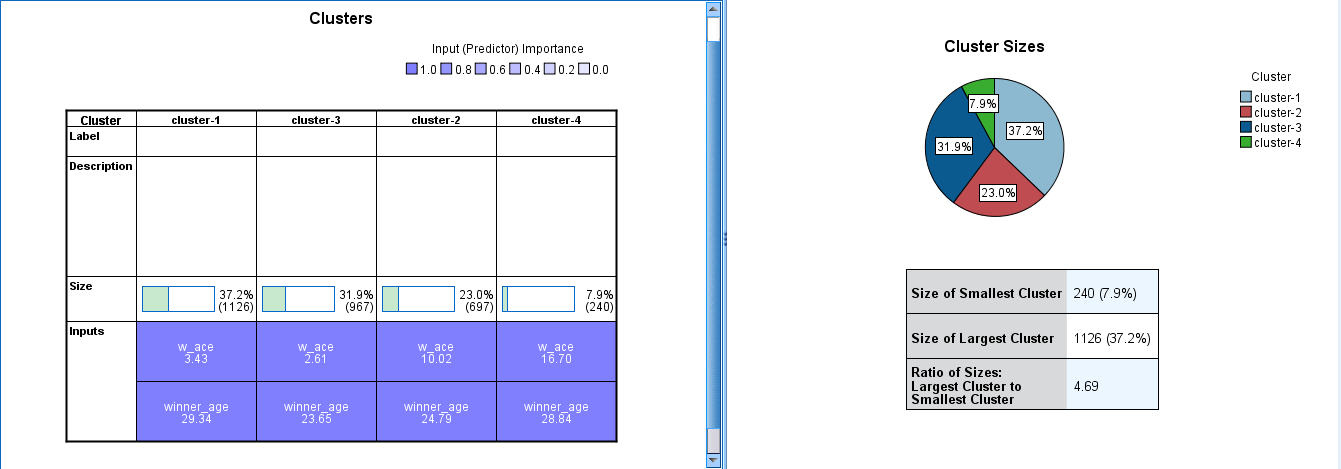
\includegraphics[scale=0.50]{Klasterovanje/Model_KMeans2011.png}
		\end{center}
		\caption{2011. godina}
		\label{fig:SPSS_Model2011}
	\end{subfigure}
	
	\vspace{0.5cm}
	\begin{subfigure}[h]{\textwidth}
		\begin{center}
			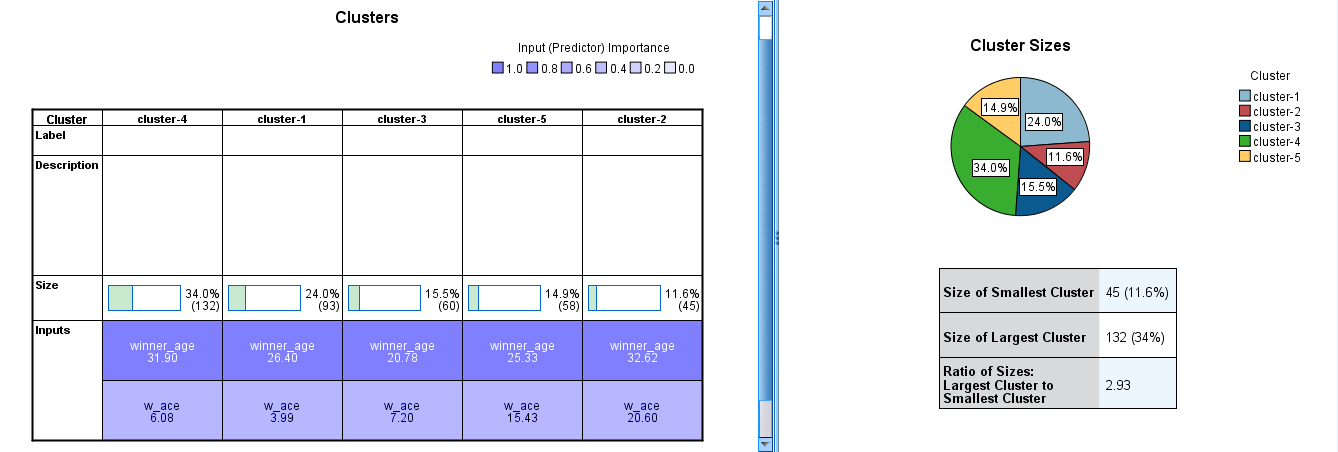
\includegraphics[scale=0.50]{Klasterovanje/Model_KMeans2017.png}
		\end{center}
		\caption{2017. godina}
		\label{fig:SPSS_Model2017}
	\end{subfigure}
	
	\caption{Modeli klastera}
	\label{ModeliKlastera}
\end{figure}

\subsection{KNIME}

\begin{figure}[H]
	\begin{center}
		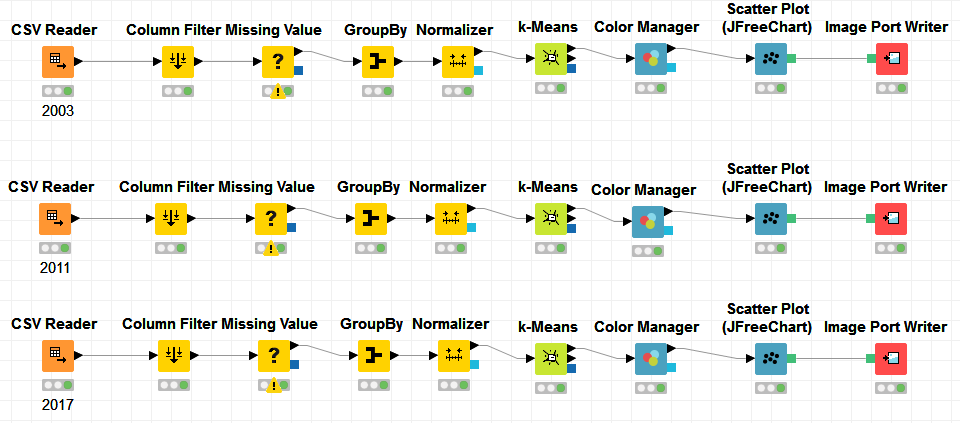
\includegraphics[scale=0.60]{Klasterovanje/KNIME_Cvorovi.png}
	\end{center}
	\caption{KNIME klasterovanje}
	\label{fig:KNIME_CvoroviKlasterovanje}
\end{figure}

U fazi pretprocesiranja podataka, otkrili smo jednog igrača sa nepoznatim brojem godina i taj red smo obrisali. U situaciji kada je broj asova bio nepoznat, stavljali smo vrednost nula. Nakon toga smo grupisali podatke po igračima, kako bi za svakog igrača dobili prosek koliko je imao asova tokom godine. Da bi iskoristili \textit{K-Means} algoritam, normalizovali smo podatke kako bi broj godina i broj asova imali isti uticaj na računanje rastojanja među instancama.  

U KNIME-u smo se opredelili da klasterovanje vršimo sa istim brojem klastera kao što smo činili u SPSS-u. Dobijeni klasteri su prikazani na slici \ref{KlasteriScatterPlot}.

\begin{figure}[H]
	\begin{subfigure}[h]{\textwidth}
		\begin{center}
			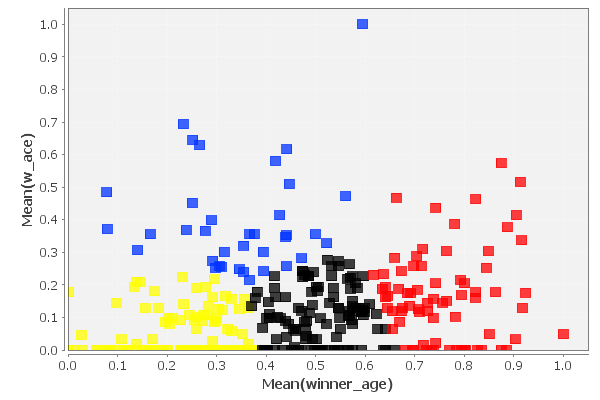
\includegraphics[scale=0.40]{Klasterovanje/ScatterPlot_KMeans2003.png}
		\end{center}
		\caption{2003. godina}
		\label{fig:KNIME_ScatterPlot2003}
	\end{subfigure}
	
	\vspace{0.5cm}
	\begin{subfigure}[h]{\textwidth}
		\begin{center}
			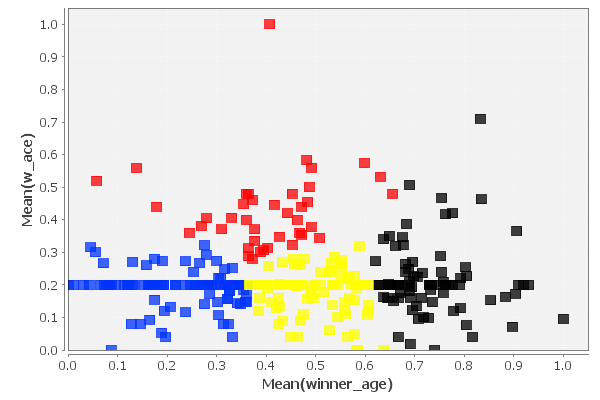
\includegraphics[scale=0.40]{Klasterovanje/ScatterPlot_KMeans2011.png}
		\end{center}
		\caption{2011. godina}
		\label{KNIME_ScatterPlot2011}
	\end{subfigure}
	
	\vspace{0.5cm}
	\begin{subfigure}[h]{\textwidth}
		\begin{center}
			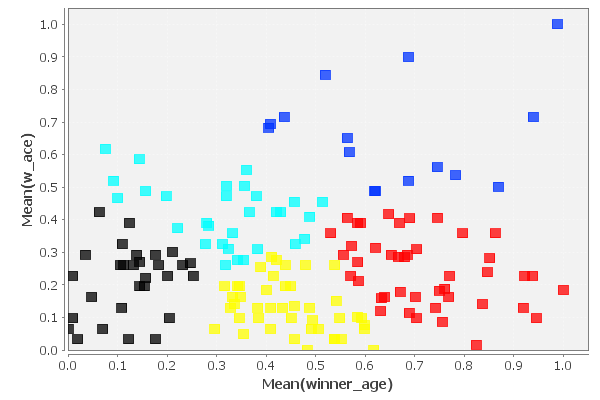
\includegraphics[scale=0.40]{Klasterovanje/ScatterPlot_KMeans2017.png}
		\end{center}
		\caption{2017. godina}
		\label{KNIME_ScatterPlot2017}
	\end{subfigure}
	
	\caption{Klasteri po godinama}
	\label{KlasteriScatterPlot}
\end{figure}

Možemo primetiti da stvarno postoje elementi van granica koji su uticali na to da se formiraju novi klasteri. Igrači koji predstavljaju elemente van granica su dati na slici \ref{fig:IgraciAutlajeri}. 

\begin{figure}[H]
	\begin{subfigure}[h]{\textwidth}
		\begin{center}
			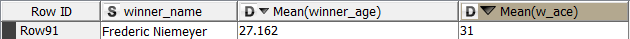
\includegraphics[scale=0.80]{Klasterovanje/FredericNiemeyer2003Outlier.png}
		\end{center}
		\caption{2003. godina}
		\label{fig:Autlajer2003}
	\end{subfigure}
	
	\vspace{0.5cm}
	\begin{subfigure}[h]{\textwidth}
		\begin{center}
			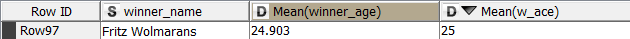
\includegraphics[scale=0.80]{Klasterovanje/FritzWolmarans2011Outlier.png}
		\end{center}
		\caption{2011. godina}
		\label{fig:Autlajer2011}
	\end{subfigure}
	
	\vspace{0.5cm}
	\begin{subfigure}[h]{\textwidth}
		\begin{center}
			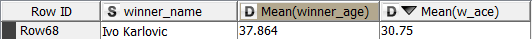
\includegraphics[scale=0.80]{Klasterovanje/IvoKarlovic2017Outlier.png}
		\end{center}
		\caption{2017. godina}
		\label{fig:Autlajer2011}
	\end{subfigure}
	
	\caption{Elementi van granica}
	\label{fig:IgraciAutlajeri}
\end{figure} 

Najinteresantiji je definitivno Ivo Karlović, koji je na meču protiv Orasia Zebaljosa na Australian Open-u postigao 75 asova. Treba imati na umu da je Karlović odigrao četiri meča na ovom turniru. Moramo napomenuti, da je skup podataka o 2017. godini nepotpun, jer je u toku te godine napravljen skup i da dosta turnira još uvek nije upisano. Trenutni skup ima samo podatke sa turnira odigranih u januaru i februaru.  


\section{Klasifikacija}

Za klasifikaciju smo odlučili da nam klase budu podloge terena, a pripadnost svakoj klasi se određuje na osnovu karakteristika četiri gubitnikova atributa (broj asova gubitnika, broj duplih servis grešaka gubitnika, broj ubačenih prvih servisa gubitnika, broj brejk šansi na servis gubitnika). Kao i kod klasterovanja i ovde smo želeli da vidimo šta se dešava u više godina. S obzirom na to da su neke podloge prisutnije u odnosu na ostale. Nakon detaljne analize raspodele podloga, odlučili smo se za 2005., 2008. i 2015. godinu. Razlog što smo odabrali baš ove godine jeste polako gubljenje ˝tepiha˝ kao podloge (slika \ref{fig:Podloga}), pa nas je zanimalo kako će ova činjenica uticati na sam proces klasifikacije. 

\begin{figure}[H]
	\begin{subfigure}[h]{\textwidth}
		\begin{center}
			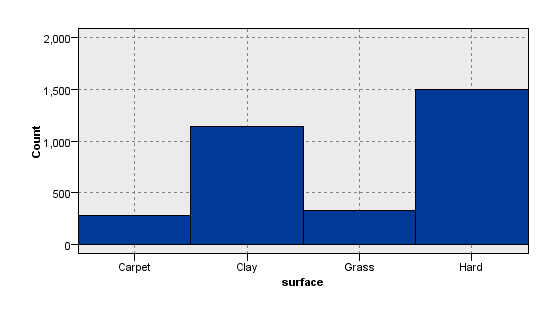
\includegraphics[scale=0.30]{Klasifikacija/HistogramiPodlogaTerena/Graphboard2005.png}
		\end{center}
		\caption{2005. godina}
		\label{fig:Podloga2005}
	\end{subfigure}

	\vspace{0.5cm}
	\begin{subfigure}[h]{\textwidth}
		\begin{center}
			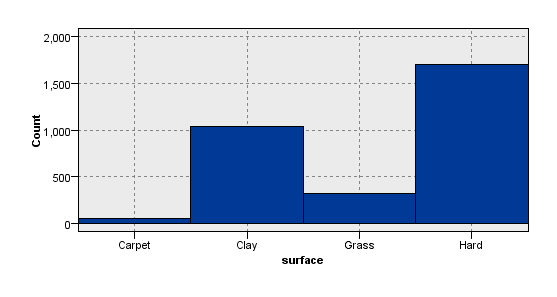
\includegraphics[scale=0.30]{Klasifikacija/HistogramiPodlogaTerena/Graphboard2008.png}
		\end{center}
		\caption{2008. godina}
		\label{fig:Podloga2008}
	\end{subfigure}

	\begin{subfigure}[h]{\textwidth}
		\begin{center}
			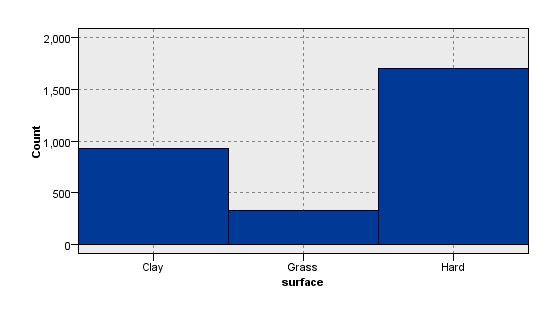
\includegraphics[scale=0.30]{Klasifikacija/HistogramiPodlogaTerena/Graphboard2015.png}
		\end{center}
		\caption{2015. godina}
		\label{fig:Podloga2015}
	\end{subfigure}
	
	\caption{Podloge terena}
	\label{fig:Podloga}
\end{figure} 

Klasifikaciju smo, takođe, obradili u SPSS-u i u KNIME-u. (slike \ref{fig:SPSS_CvoroviKlasifikacija} i \ref{fig:KNIME_CvoroviKlasifikacija}).

\subsection{SPSS}

\begin{figure}[H]
	\begin{center}
		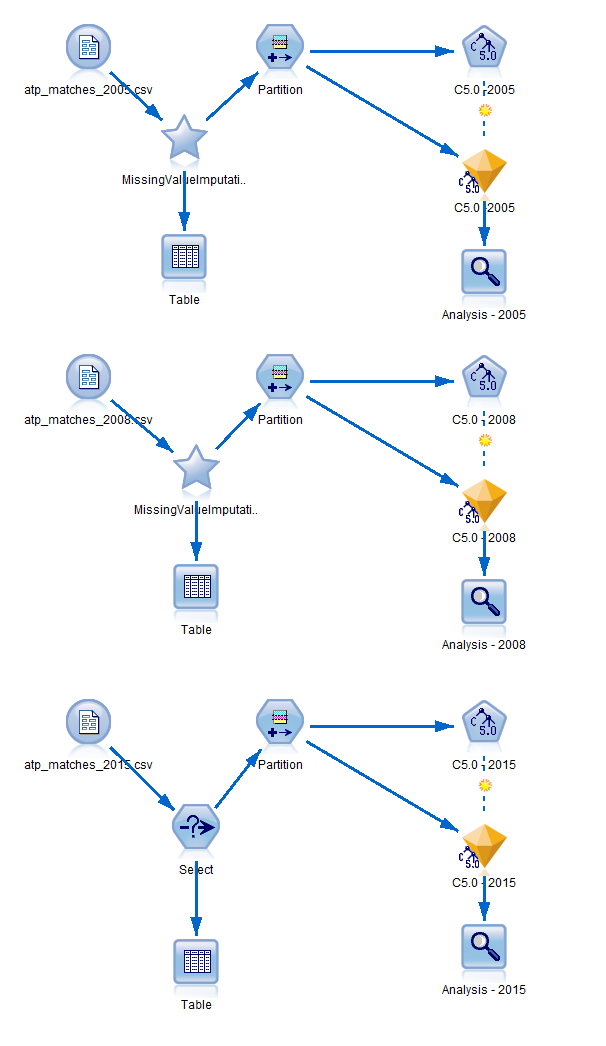
\includegraphics[scale=0.60]{Klasifikacija/C50/SPSS_C50_Surface.png}
	\end{center}
	\caption{SPSS klastifikacija}
	\label{fig:SPSS_CvoroviKlasifikacija}
\end{figure}

Primenili smo \textit{C5.0} algoritam sa podelom na trening i test skup u odnosu 70-30. Na slici \ref{fig:ModelKlasifikacijaC50} možemo videti analizu najvažnijjih atributa. Najvažniji atribut je u sve tri godine broj asova, ono što je interesantno jeste da je u 2008. godini važnost ˝broja duplih grešaka˝ nešto malo iznad nule {\color{red}Nađi tačan broj}, a u 2015. godini uopšte nije ni uzet u razmatranje.

\begin{figure}[H]
	\begin{subfigure}[h]{\textwidth}
		\begin{center}
			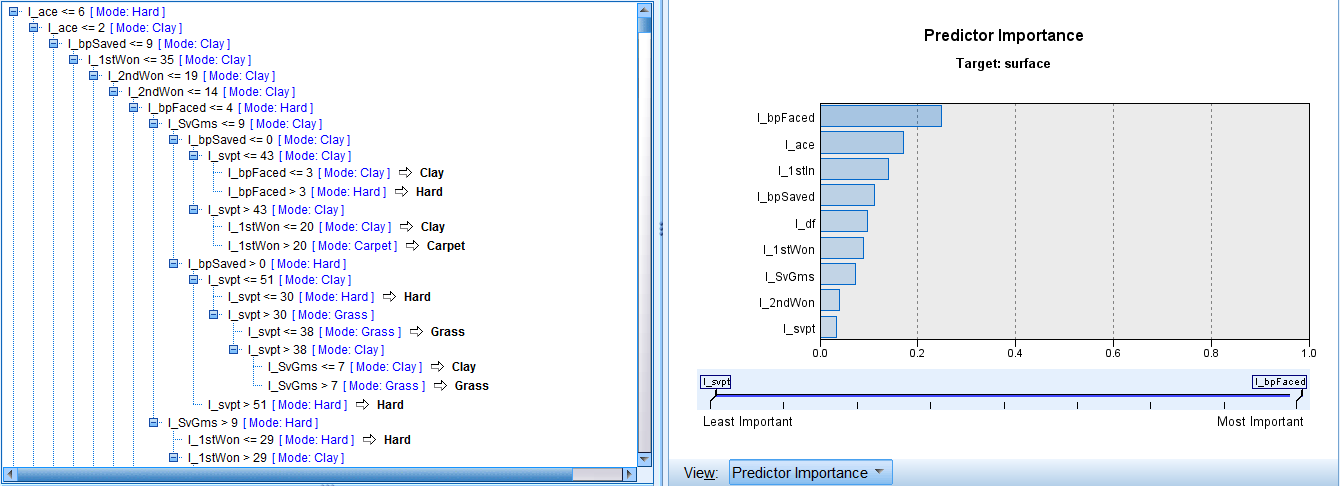
\includegraphics[scale=0.50]{Klasifikacija/C50/Model_Surface2005.png}
		\end{center}
		\caption{2005. godina}
		\label{fig:ModelKlasifikacijaC502005}
	\end{subfigure}
	
	\vspace{0.5cm}
	\begin{subfigure}[h]{\textwidth}
		\begin{center}
			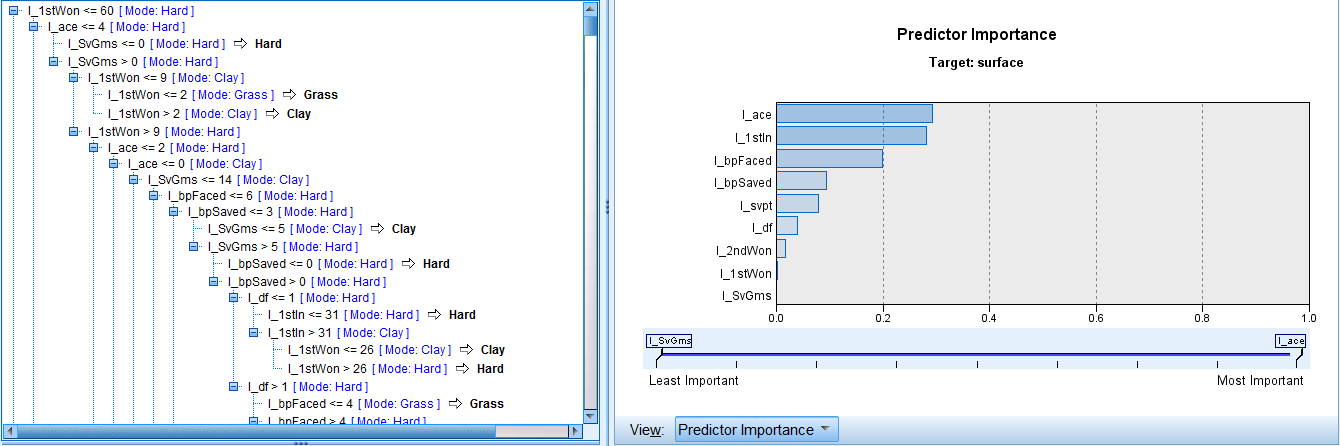
\includegraphics[scale=0.50]{Klasifikacija/C50/Model_Surface2008.png}
		\end{center}
		\caption{2008. godina}
		\label{fig:ModelKlasifikacijaC502008}
	\end{subfigure}
	
	\vspace{0.5cm}
	\begin{subfigure}[h]{\textwidth}
		\begin{center}
			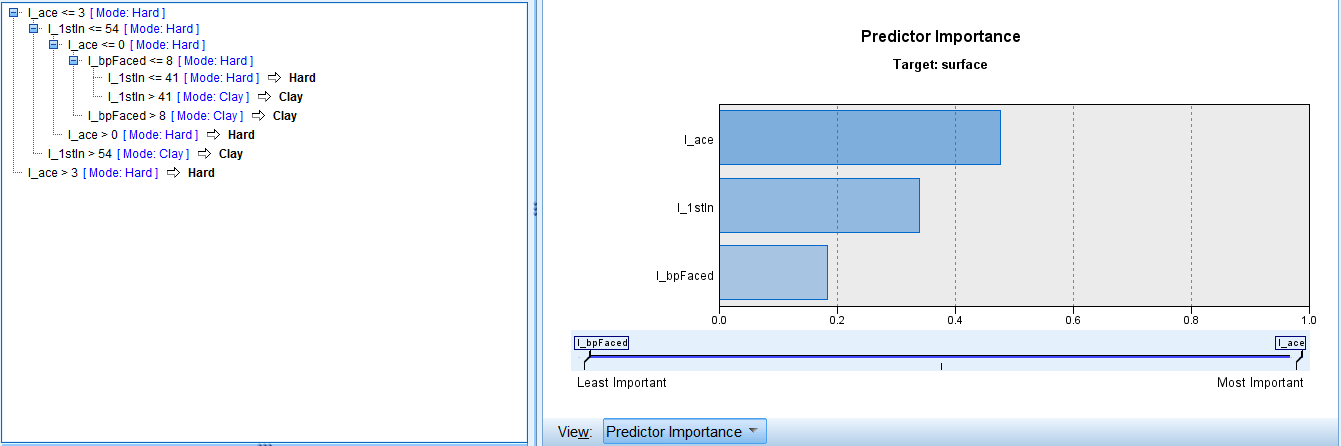
\includegraphics[scale=0.50]{Klasifikacija/C50/Model_Surface2015.png}
		\end{center}
		\caption{2015. godina}
		\label{fig:ModelKlasifikacijaC502015}
	\end{subfigure}
	
	\caption{Model klasifikacije}
	\label{fig:ModelKlasifikacijaC50}
\end{figure}

Drveta odlučivanja smo delom mogli da vidimo i na prethodnoj slici, a detaljniji prikaz se može pogledati: \href{file:./Klasifikacija/C50/Model_Surface2005.html}{2005}, \href{file:./Klasifikacija/C50/Model_Surface2008.html}{2008}, \href{file:./Klasifikacija/C50/Model_Surface2005.html}{2015}. 

Intuitivan prikaz drveta odlučivanja za 2005. i 2008. godinu, i kompletan prikaz 2015.godine može se videti na slici \ref{fig:DrvoOdlucivanjaC50}.

\begin{figure}[H]
	\begin{subfigure}[h]{\textwidth}
		\begin{center}
			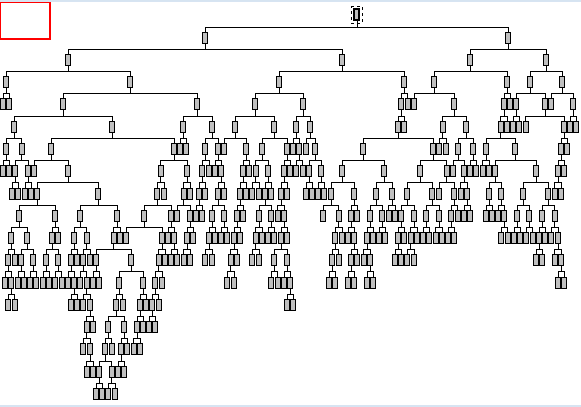
\includegraphics[scale=0.35]{Klasifikacija/C50/MapaDrvetaOdlucivanja2005.png}
		\end{center}
		\caption{2005. godina}
		\label{fig:DrvoOdlucivanjaC502005}
	\end{subfigure}

	\vspace{0.5cm}
	\begin{subfigure}[h]{\textwidth}
		\begin{center}
			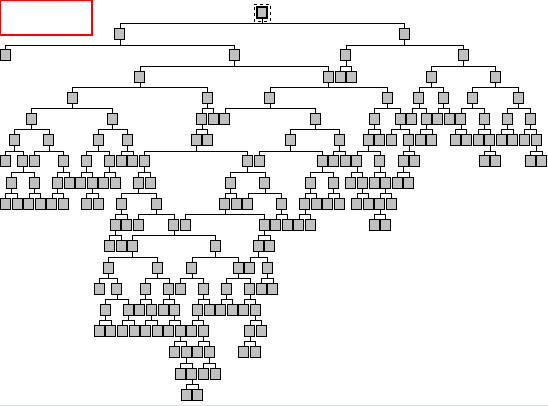
\includegraphics[scale=0.50]{Klasifikacija/C50/MapaDrvetaOdlucivanja2008.png}
		\end{center}
		\caption{2008. godina}
		\label{fig:DrvoOdlucivanjaC502008}
	\end{subfigure}
	
	\vspace{0.5cm}
	\begin{subfigure}[h]{\textwidth}
		\begin{center}
			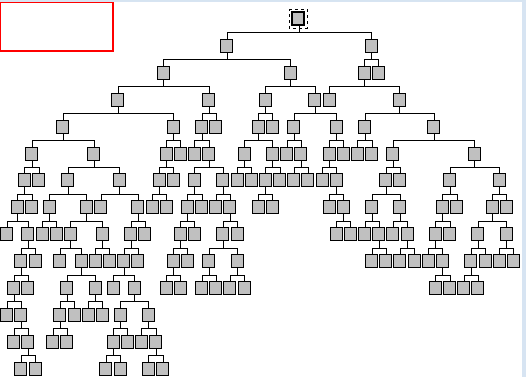
\includegraphics[scale=0.60]{Klasifikacija/C50/MapaDrvetaOdlucivanja2015.png}
		\end{center}
		\caption{2015. godina}
		\label{fig:DrvoOdlucivanjaC502015}
	\end{subfigure}
	
	\caption{Drveta odlučivanja C-5.0}
	\label{fig:DrvoOdlucivanjaC50}
\end{figure}

Kao što možemo da vidimo da su drveta iz 2005 i 2008 ogromna, dok je {\color{red}Ovo iz 2015 bi mogli da izanaliziramo...}

Dobijena preciznost, a i matrica konfuzije su prikazane na slici \ref{fig:MatricaKnfuzijeC50}.

\begin{figure}[H]
	\begin{subfigure}[h]{\textwidth}
		\begin{center}
			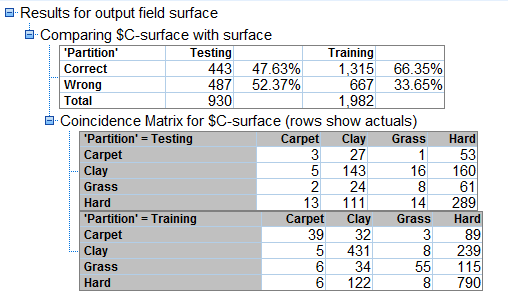
\includegraphics[scale=0.50]{Klasifikacija/C50/Analysis_Surface2005.png}
		\end{center}
		\caption{2005. godina}
		\label{fig:MatricaKnfuzijeC502005}
	\end{subfigure}

	\vspace{0.5cm}
	\begin{subfigure}[h]{\textwidth}
		\begin{center}
			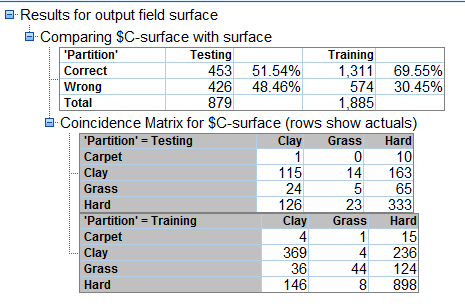
\includegraphics[scale=0.45]{Klasifikacija/C50/Analysis_Surface2008.png}
		\end{center}
		\caption{2008. godina}
		\label{fig:MatricaKnfuzijeC502008}
	\end{subfigure}
	
	\begin{subfigure}[h]{\textwidth}
		\begin{center}
			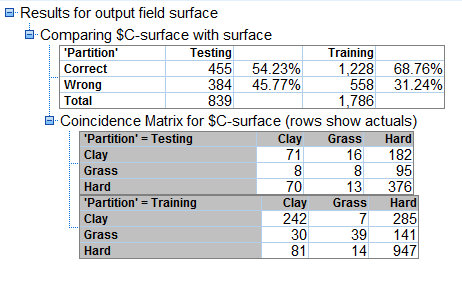
\includegraphics[scale=0.50]{Klasifikacija/C50/Analysis_Surface2015.png}
		\end{center}
		\caption{2015. godina}
		\label{fig:MatricaKnfuzijeC502015}
	\end{subfigure}
	
	\caption{Matrice konfuzije - C5.0}
	\label{fig:MatricaKnfuzijeC50}
\end{figure}

Možemo da primetimo da se ˝tepih˝ klasifikuje kao ˝beton˝, što je i očekivano s obzirom na odnos turinara odigranih na ova dva turnira. Takođe treba primetiti da se i ˝trava˝ u 2015. godini gotovo uvek klasifikuje kao ˝beton˝, a nikad kao ˝trava˝. Možemo da primetimo i da nam je preciznost zajedno sa godinama postepeno rasla, ali nismo baš zadovoljni dobijenim rezultatima pa smo odlučili da ispitamo metodu Drveta odlučivanja i u KNIME-u. 

Sveobuhvatni prikaz rada algoritma C5.0 dat je u fajlovima: \href{file:./Klasifikacija/C50/Summary_Surface2005.html}{2005}, \href{file:./Klasifikacija/C50/Summary_Surface2008.html}{2008}, \href{file:./Klasifikacija/C50/Summary_Surface2005.html}{2015}.  

S obzirom da su nam dobijeni rezultati algoritma C-5.0 dosta šarenoliki, i dobijena preciznost i veličina drveta odlučivanja nam deluju kao da se desilo preprilagođavanje odlučili smo da na godine 2005 i 2015 izvršimo istu analizu u alatu KNIME.

\subsection{KNIME}

U alatu  KNIME smo za klasifikaciju koristili Drveta odlučivanja, K najbližih suseda i metod potpornih vektora (SVM)

\subsubsection{Drveta odlučivanja}

\begin{figure}[h!]
	\begin{center}
		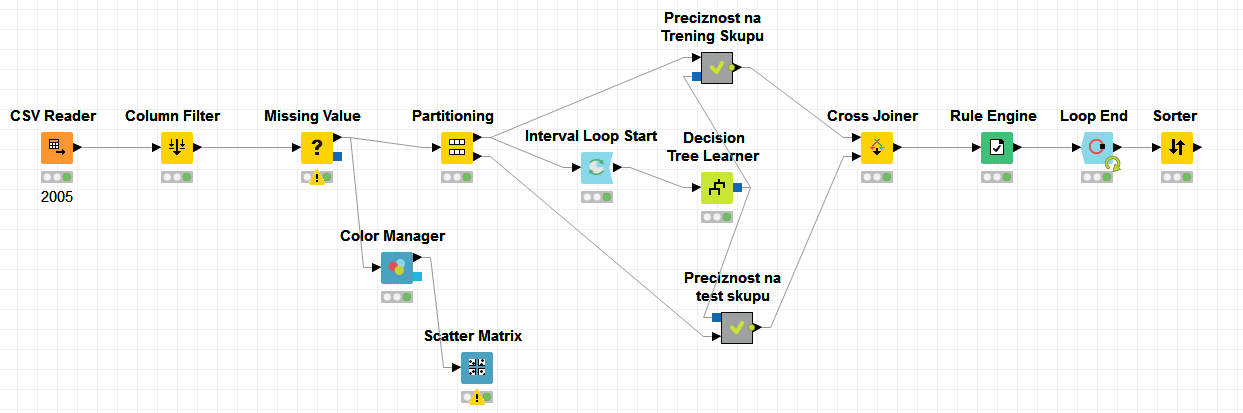
\includegraphics[scale=0.45]{Klasifikacija/DrvoOdlucivanja/KNIME_DrvoOdlucivanjaCvorovi.png}
	\end{center}
	\caption{KNIME implementacija tehnike Drvo odlučivanja}
	\label{fig:KNIME_CvoroviKlasifikacija}
\end{figure}

Pre same klasifikacije na slici \ref{fig:KlasifikacijaScatterMatrix} je prikazan je odnos između atributa klasterovanja.

\begin{figure}[H]
	\begin{subfigure}[h]{\textwidth}
		\begin{center}
			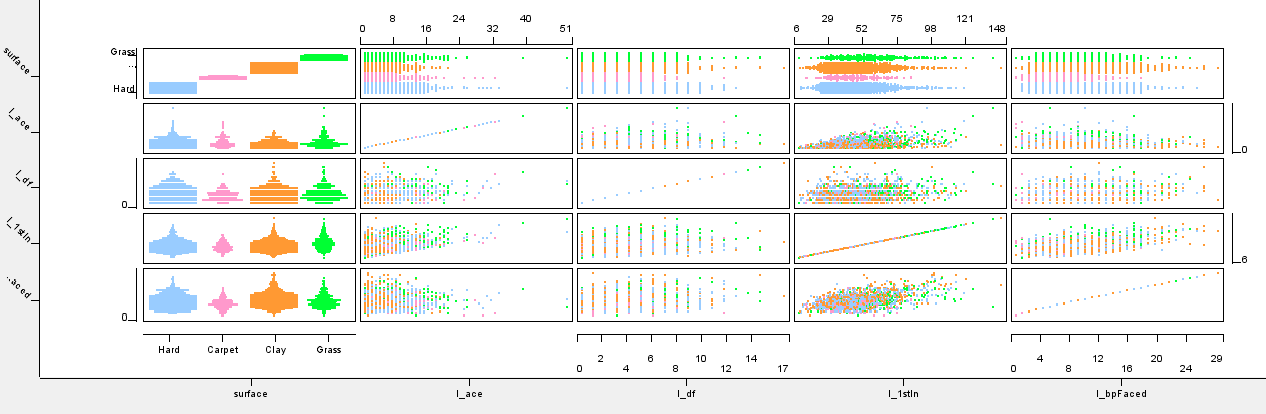
\includegraphics[scale=0.45]{Klasifikacija/DrvoOdlucivanja/2005/Korelacija.png}
		\end{center}
		\caption{2005. godina}
		\label{fig:KlasifikacijaScatterMatrix2005}
	\end{subfigure}
	
	\vspace{0.5cm}
	\begin{subfigure}[h]{\textwidth}
		\begin{center}
			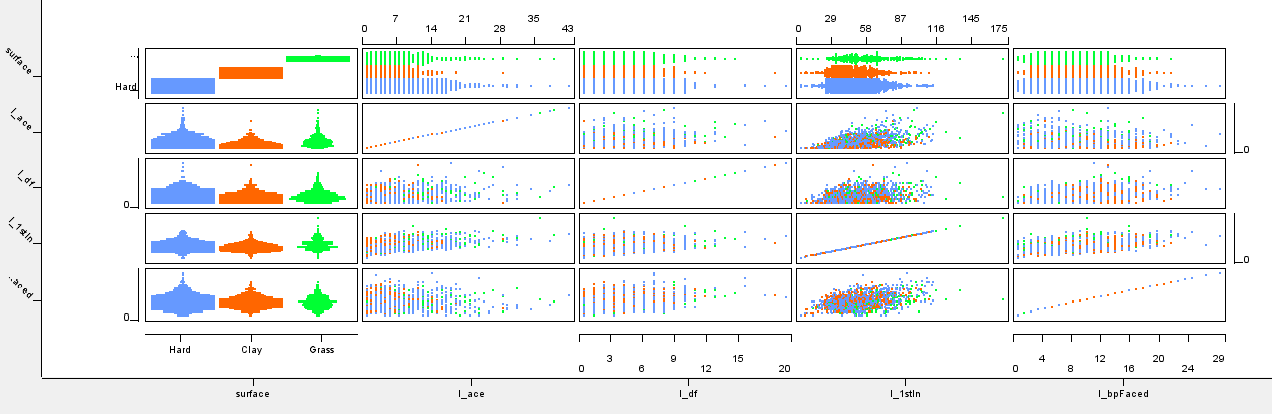
\includegraphics[scale=0.45]{Klasifikacija/DrvoOdlucivanja/2015/Korelacija.png}
		\end{center}
		\caption{2008. godina}
		\label{fig:KlasifikacijaScatterMatrix2015}
	\end{subfigure}
	
	\caption{Korelacija atributa}
	\label{fig:KlasifikacijaScatterMatrix}
\end{figure}

Dobijena preciznost, a i matrica konfuzije su prikazane na slikama \ref{fig:MatricaKnfuzije2005} i \ref{fig:MatricaKnfuzije2015}.

\begin{figure}[H]
	\begin{subfigure}[h]{\textwidth}
		\begin{center}
			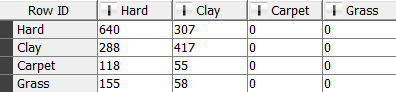
\includegraphics[scale=0.60]{Klasifikacija/DrvoOdlucivanja/2005/MatricaKonfuzijeTrening.png}
		\end{center}
		\label{fig:MatricaKnfuzijeTrening2005}
	\end{subfigure}

	\vspace{0.5cm}
	\begin{subfigure}[h]{\textwidth}
		\begin{center}
			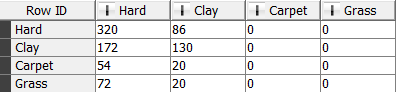
\includegraphics[scale=0.60]{Klasifikacija/DrvoOdlucivanja/2005/MatricaKonfuzijeTest.png}
		\end{center}
		\label{fig:MatricaKnfuzijeTest2005}
	\end{subfigure}
	\caption{Matrice konfuzije - 2005}
	\label{fig:MatricaKnfuzije2005}
\end{figure}

\begin{figure}[H]
	\begin{subfigure}[h]{\textwidth}
		\begin{center}
			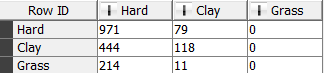
\includegraphics[scale=0.60]{Klasifikacija/DrvoOdlucivanja/2015/MatricaKonfuzijeTrening.png}
		\end{center}
		\label{fig:MatricaKnfuzijeTrening2015}
	\end{subfigure}

	\vspace{0.5cm}
	\begin{subfigure}[h]{\textwidth}
		\begin{center}
			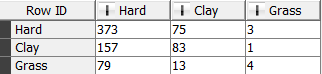
\includegraphics[scale=0.60]{Klasifikacija/DrvoOdlucivanja/2015/MatricaKonfuzijeTest.png}
		\end{center}
		\label{fig:MatricaKnfuzijeTest2015}
	\end{subfigure}
	\caption{Matrice konfuzije - 2015}
	\label{fig:MatricaKnfuzije2015}
\end{figure}
\begin{figure}
	\begin{subfigure}[h]{\textwidth}
		\begin{center}
			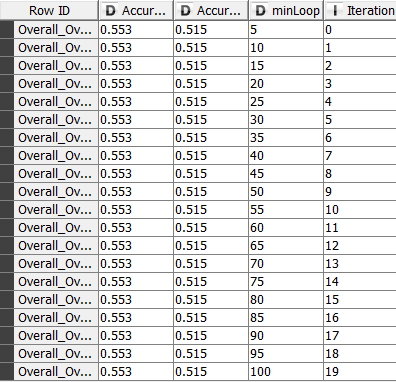
\includegraphics[scale=0.75]{Klasifikacija/DrvoOdlucivanja/2005/Preciznost.png}
		\end{center}
		\caption{2005. godina}
		\label{fig:Preciznost2005}
	\end{subfigure}

	\vspace{0.5cm}
	\begin{subfigure}[h]{\textwidth}
		\begin{center}
			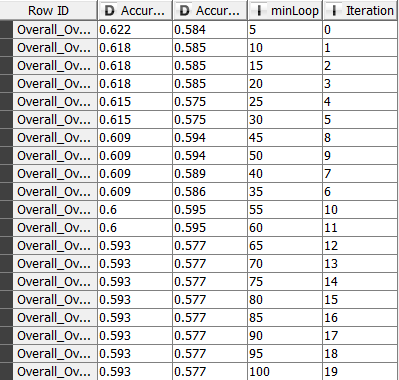
\includegraphics[scale=0.75]{Klasifikacija/DrvoOdlucivanja/2015/Preciznost.png}
		\end{center}
		\caption{2015. godina}
		\label{fig:Preciznost2015}
	\end{subfigure}
	
	\caption{Preciznost}
	\label{fig:PreciznostKNIME}
\end{figure}

\subsubsection{SVM}

\begin{figure}[h!]
	\begin{center}
		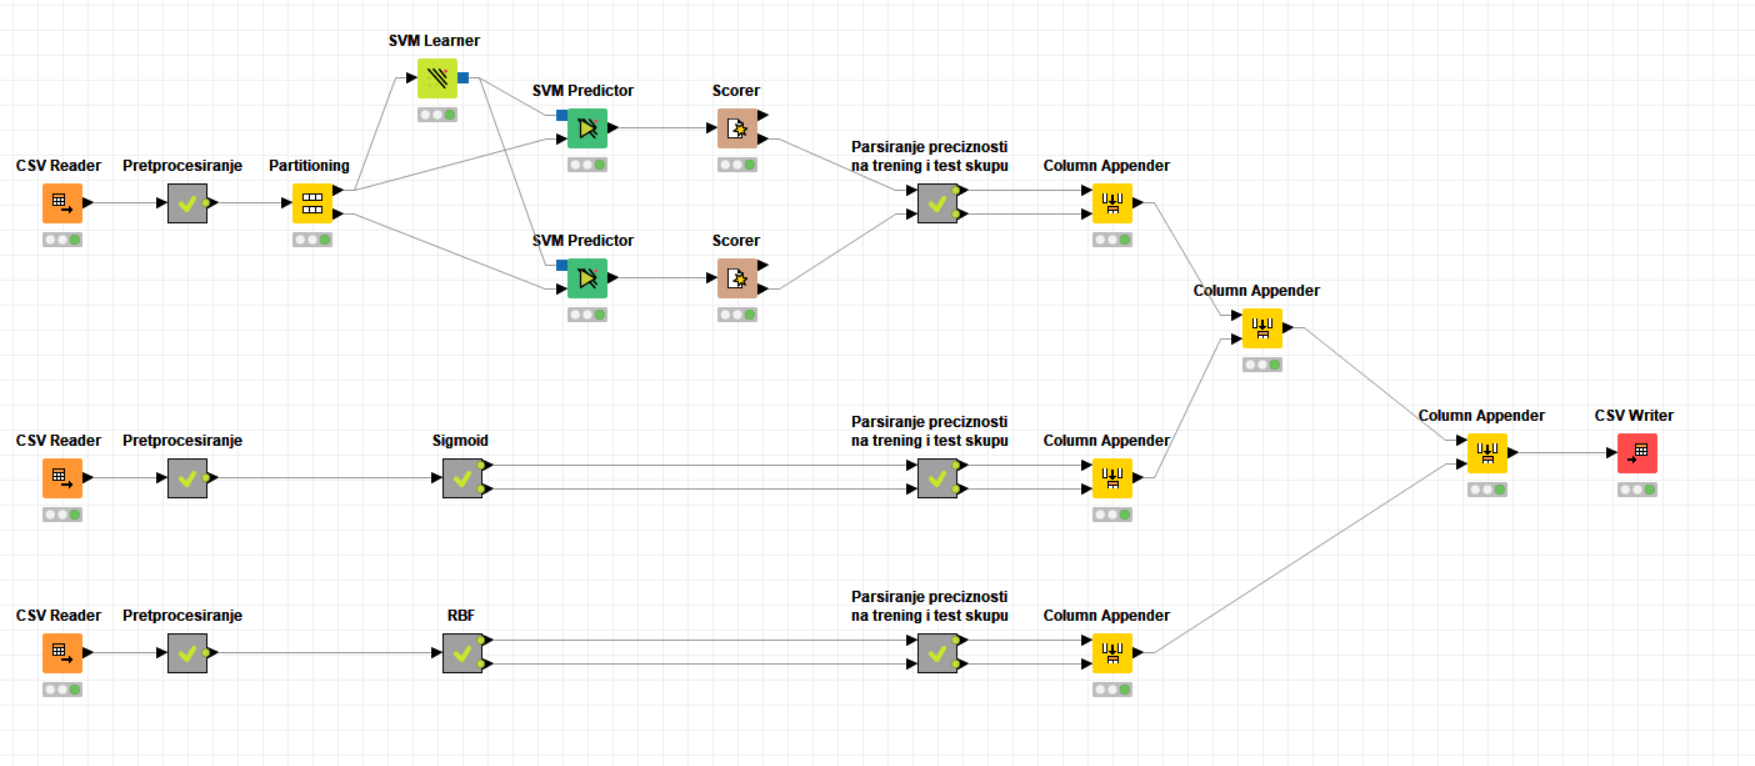
\includegraphics[scale=0.30]{KNIME_project/SVM/SVM_knime}
	\end{center}
	\caption{KNIME implementacija SVM tehnike}
	\label{fig:KNIME_CvoroviKlasifikacija}
\end{figure}

Vršili smo klasifikaciju tehnikom \textit{SVM}. Normalizovane podatke smo podelili na trening i test skup u odnosu 70-30.
Primenili smo sva tri raspoloživa kernela (polinomijalni trećeg stepena, sigmoid, Gausov(RBF)).
Na slici \ref{fig:precision} se mogu videti preciznosti za sva tri kernela, i za trening i za test skup.

\begin{figure}[h!]
	\begin{center}
		
\includegraphics[scale=0.45]{KNIME_project/SVM/preciznost}
	\end{center}
	\caption{Preciznost za različite kernele}
	\label{fig:precision}
\end{figure}


Koristeći polinomijalni kernel trećeg stepena, dobili smo izuzetno loše rezultate.
Naime, skoro 50\% redova (1501 od 3257) odgovaraju mečevima koji su odigrani na tvrdoj podlozi.
Na slikama \ref{fig:poly_training} i \ref{fig:poly_test} vidimo da su podaci pogrešno klasifikovani u
mečeve koji su odigrani na šljaci.

\begin{figure}[h!]
	\begin{center}
		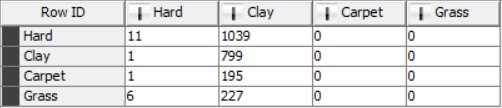
\includegraphics[scale=0.80]{KNIME_project/SVM/poly_training}
	\end{center}
	\caption{Trening podaci za polinomijalni kernel}
	\label{fig:poly_training}
\end{figure}

\begin{figure}[h!]
	\begin{center}
		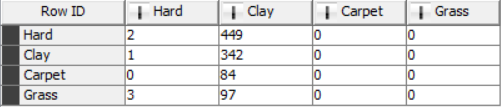
\includegraphics[scale=0.80]{KNIME_project/SVM/poly_test}
	\end{center}
	\caption{Test podaci za polinomijalni kernel}
	\label{fig:poly_test}
\end{figure}

%\newpage

Koristeći sigmoid kernel, situacija se promenila utoliko što su podaci vezani za tvrdu podlogu
vrlo dobro klasifikovani, što se može videti na slikama \ref{fig:sigmoid_training} i \ref{fig:sigmoid_test}.
Primetimo da su podaci uglavnom raspoređeni u klase koje se odnose na beton i šljaku.

\begin{figure}[h!]
	\begin{center}
		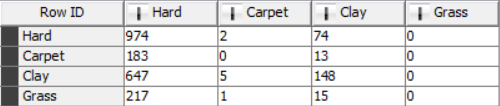
\includegraphics[scale=0.80]{KNIME_project/SVM/sigmoid_training}
	\end{center}
	\caption{Trening podaci za sigmoid kernel}
	\label{fig:sigmoid_training}
\end{figure}

\begin{figure}[h!]
	\begin{center}
		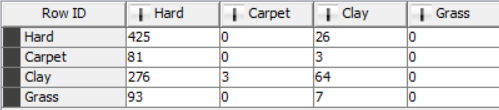
\includegraphics[scale=0.80]{KNIME_project/SVM/sigmoid_test}
	\end{center}
	\caption{Test podaci za sigmoid kernel}
	\label{fig:sigmoid_test}
\end{figure}

Koristeći Gausov kernel, dobili smo lošiju klasifikaciju za tvrdu podlogu, dosta bolju klasifikaciju za šljaku
i malo bolju klasifikaciju za travu (slike \ref{fig:rbf_training} i \ref{fig:rbf_test}). \\

\begin{figure}[h!]
	\begin{center}
		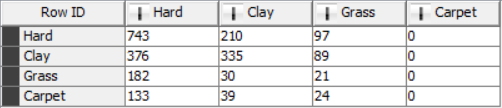
\includegraphics[scale=0.80]{KNIME_project/SVM/rbf_training}
	\end{center}
	\caption{Trening podaci za Gausov kernel}
	\label{fig:rbf_training}
\end{figure}

\begin{figure}[h!]
\begin{center}
	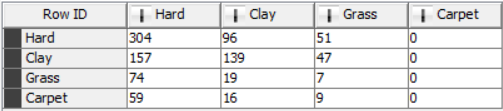
\includegraphics[scale=0.80]{KNIME_project/SVM/rbf_test}
\end{center}
\caption{Test podaci za Gausov kernel}
\label{fig:rbf_test}
\end{figure}

Prikazani rezultati su za 2005. godinu i, kako je u svim slučajevima klasifikacija koja se odnosila na tepih davala nulu, slični rezultati su očekivani i za 2008. godinu. Stoga nismo obrađivali ostale godine \textit{SVM} metodom, već smo pokušali da obradimo podatke algoritmom \textit{C5.0} u SPSS-u.

\end{document}